%\newpage
%\end{multicols}\begin{multicols}{2}
\subsection{Quo vadis studens? - Einige Worte zum Bachelor}

% TODO Ich (Brian) meine ja immernoch, so nagelneu ist die nicht. Sie wurde überarbeitet, mehr aber nicht.
Der diesj"ahrige Erstsemesterjahrgang --- ja, genau, damit seid ihr
gemeint --- ist der Erste, der zum Sommersemester unseren Bachelor
beginnen darf. Dazu gehört auch ein nagelneuer, noch originalverpackter
und fr"uhlingsfrisch duftender Musterstudienplan, den ihr
erduld \dots befolgen könnt.
% Pr"ufungsordnung erleid... err.. %genie"sen darf.
Außerdem habt ihr das große Vergnügen, als zweiter Jahrgang eine neue 
%Mit der neuen 
Pr"ufungsordnung genießen zu dürfen. Mit ihr  wird im Vergleich zu den vorangegangenen
Jahrg"angen einiges einfacher, einiges nerviger, vor allem aber einiges flexibler. 

Da stellt sich
zwangsl"aufig die Frage, wie man sein Studium plant, schlie"slich will
man in 3 Jahren (Bachelor) oder 2 Jahren (Master) mit seinem
Abschluss wieder aus dieser Anstalt raus und nicht pl"otzlich merken, dass man diese und jene
Pr"ufungsleistung noch nicht erbracht hat. 
%\footnote{Dieser Text bezieht
%sich in erster Linie auf den Bachelor, zum Master siehe \ref{master} auf
%\pageref{master}.}
Wie ihr sicherlich bemerkt habt, ist die Pr"ufungsordnung euer wichtigstes Dokument, das euch
durchs Studium begleiten wird und euch vorschreibt, was ihr zu tun und zu lassen habt. Sie ist bei
uns die dritte Pr"ufungsordnung, die sich am Bologna-Prozess orientiert, wodurch ihr theoretisch
eure Leistungen mit allen Universit"aten, die ebenfalls einen Bachelor/Master nach Bologna
anbieten, vergleichen k"onnt. In der Praxis mag das jedoch anders aussehen *hust*.

Grunds"atzlich schreibt die Pr"ufungsordnung 180 Leistungspunkte f"ur
den Bachelor- und 120 Leistungspunkte für den Master-Abschluss vor.
Die d"urft ihr aber nicht einfach so durch Vorlesungen erreichen, die euch gefallen, sondern es gibt
bestimmte Pflichtveranstaltungen, die belegt werden m"ussen. Dazu
z"ahlen im Bachelor beispielsweise Vorlesungen wie Logik und Anaylsis, um die
ihr in den 1. Semestern des Bachelors nicht herumkommen werdet. Au"serdem muss im Laufe des Studiums ein Seminar, ein
Teamprojekt und auch das ber"uhmt ber"uchtigte Softwareentwicklungspraktikum absolviert werden.
Zur wirklich freien Auswahl stehen das Nebenfach und der informatische und mathematische
Wahlpflichtbereich. Letzterer muss 10 Leistungspunkte umfassen (das sind 2 Vorlesungen),
w"ahrend im Nebenfach 14 bis 18 und im Informatik-Bereich 20 bis 24 Punkte erreicht werden
m"ussen.

Doch was f"angt man jetzt damit an? W"ahrend ihr euch am Anfang eures Studiums sicherlich
erstmal mit den Pflichtf"achern besch"aftigen werdet (nicht zuletzt, weil die auch im
Musterstudienplan in den ersten drei Semestern stehen), lohnt es sich trotzdem, sich schon am
Anfang des Studiums damit auseinanderzusetzen, was man hier in Braunschweig "uberhaupt so
machen kann. Interessant ist auch, wann man es machen kann. So werden einige
Wahlpflichtveranstaltungen nur alle zwei Jahre angeboten. Oder man kann das Nebenfach nur in
Wintersemestern h"oren und m"ochte dann vielleicht im Sommersemester doppelt so viel Informatik
h"oren.

Wichtig ist vor allem auch, dass die speziell f"ur den Bachelor angebotenen Vorlesungen stark
gek"urzt wurden, da viele, die fr"uher im Bachelor waren, nun in den Master verschoben wurden. Das
ist f"ur euch jedoch kein Nachteil, denn als Bachelor kann man Master-Vorlesungen auf Antrag
bereits in den Bachelor einbringen. Daf"ur reicht es in der Regel, einfach einen formlosen Antrag
beim Pr"ufungsausschuss zu stellen, in dem ihr sagt, dass ihr gerne diese und jene Vorlesung im
Bachelor einbringen m"ochtet. Anschlie"send zur Pr"ufung anmelden und bestehen, mehr nicht. 
Umgekehrt ist dies i.d.R. nicht möglich, also kann ein Masterstudent keine Bachelor-Vorlesungen in sein Studium einbringen. 
In begründeten Ausnahmefällen geht aber sogar das, wozu ebenfalls ein Antrag zu stellen ist.

Wie ihr seht, seid ihr mit eurem Studium recht flexibel, und es wird hier auch niemanden geben, der
euch vorschreibt, wann ihr zu welchen Vorlesungen gehen m"usst oder das in irgendeiner Weise
kontrolliert und euch daran erinnert. Ihr erlangt euren Abschluss, wenn ihr alle Voraussetzungen aus
der Pr"ufungsordnung erf"ullt. Und wenn ihr im 6. Semester immer noch eine Pflichtpr"ufung offen
habt, dann ist das einzig und allein euer Problem.\footnote{Bzw., wenn ihr bewusst eingeplant habt, länger zu studieren, ist es eben kein Problem.} 

Der Musterstudienplan, den ihr zum Beispiel bei Herrn Dr. Struckmann
oder Frau Sehnert bekommen k"onnt, wenn ihr
ihn noch nicht habt, bietet schon mal einen sehr guten roten Faden, an dem man sich entlanghangeln
kann und dann sicher sein kann, dass man nach 6 Semestern alles hat, was man braucht. Allerdings
solltet ihr wissen, dass die Pflichtvorlesungen dieses Semester gegen"uber den vorangegangenen fast
alle im Wert hochgesetzt wurden und eure Vorg"anger zus"atzlich in den ersten beiden Semestern
noch Technische und Theoretische Informatik 1 und 2 geh"ort haben. Das ist der Grund daf"ur,
warum euer Stundenplan auf den ersten Blick etwas mager ausfallen wird. Aber weil wir nun die
ersten fertigen Bachelor-Absolventen haben und ein wenig mehr Erfahrung mit den h"oheren
Semester haben, haben wir uns f"ur euch einen alternativen Studienplan
"uberlegt (Seite \pageref{studienplan_neu}).

Diesen empfehlen wir nat"urlich nur denen, die sich den geringen Mehraufwand pro Semester zutrauen. Ihr werdet es
sehr genie"sen, w"ahrend des SEPs und der Bachelorarbeit nicht so viele Vorlesungen zu haben, die
eure Zeit rauben. Und mit entsprechendem Talent schafft man auch die paar Credits mehr in den
anderen Semestern. Wir halten nat"urlich diesen alternativen Studienplan f"ur ausgewogener und
studentenfreundlicher als den, den die Fakult"at euch zur Verf"ugung stellt, aber auch er ist nur eine
Empfehlung. Ihr seid nicht mehr in der Schule, ihr habt nun Freiheiten, nutzt sie weise und studiert
so, wie ihr es f"ur richtig haltet.


\end{multicols}
%\begin{wrapfigure}{l}{\linewidth}
    \begin{center}
          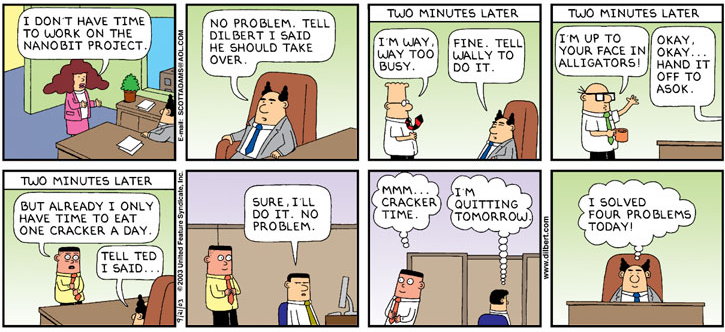
\includegraphics[width=\linewidth]
	  {bilder/comics/dilbert.png}    \end{center}
%	\end{wrapfigure}
	\begin{multicols}{2}

%%% Local Variables: 
%%% mode: latex
%%% TeX-master: "../../1-te"
%%% End: 
